\documentclass{beamer}
\usepackage{remreset} % For adding header dots
\usepackage{utopia} % Fonts
\usepackage{csquotes} % Quotes
\usepackage{xcolor} % Colors
\usetheme{Frankfurt}
\usecolortheme{default}
\definecolor{darkred}{rgb}{0.7,0,0} % Set darkred shortcut
\setbeamercolor{structure}{fg=darkred!90!black} % Change theme colors
\setbeamercolor{bibliography item}{parent=palette primary}
\setbeamercolor*{bibliography entry title}{parent=palette primary}
\def\code#1{\texttt{#1}} % Define code shortcut

% Custom footer for the presentation
\makeatother
\setbeamertemplate{footline}{
  \leavevmode%
  \hbox{%
  \begin{beamercolorbox}[wd=.4\paperwidth,ht=2.25ex,dp=1ex,center]{author in head/foot}%
    \usebeamerfont{author in head/foot}\insertshortauthor\expandafter\ifblank\expandafter{\beamer@shortinstitute}{}{~~(\insertshortinstitute)}
  \end{beamercolorbox}%
  \begin{beamercolorbox}[wd=.3\paperwidth,ht=2.25ex,dp=1ex,center]{title in head/foot}%
    \usebeamerfont{title in head/foot}\insertshorttitle
  \end{beamercolorbox}%
  \begin{beamercolorbox}[wd=.3\paperwidth,ht=2.25ex,dp=1ex,right]{date in head/foot}%
    \usebeamerfont{date in head/foot}\insertshortdate{}\hspace*{2em}
    \insertframenumber{} / \inserttotalframenumber\hspace*{2ex} 
  \end{beamercolorbox}}%
  \vskip0pt%
}
\setcounter{subsection}{1}

% Remove navigation symbols and add dots in header
\makeatletter
\setbeamertemplate{navigation symbols}{}
\@removefromreset{subsection}{section}

% Put Table of Contents before each section
\AtBeginSection[]
{
  \begin{frame}
    \frametitle{Table of Contents}
    \tableofcontents[currentsection]
  \end{frame}
}

% Infos
\title[The Rcpp Package] {The Rcpp Package}
\subtitle{An Introduction}
\author[Sarti, Milite, Scassola] {Gabriele Sarti \and Salvatore Milite \and Davide Scassola}
\institute[UniTs] 
{
    University of Trieste \\
    Department of Mathematics and Geosciences

    \begin{figure}[htb]
        \centering
        \begin{minipage}{0.45\textwidth}
            \centering
            
\includegraphics[width=0.4\textwidth]{units.png}
        \end{minipage}
        \begin{minipage}{0.45\textwidth}
            \centering
            
\includegraphics[width=0.8\textwidth]{logo-dssc.png}
        \end{minipage}
    \end{figure}
    \vspace{-5mm}
}
\date[June 26th, 2019] {Statistical Methods for Data Science Final Exam \\ June 26th, 2019}

\begin{document}

% Title page.
\frame{\titlepage}


% TOC after title page
\begin{frame}
\frametitle{Table of Contents}
\tableofcontents
\end{frame}

%-----------------------------------

\section{The R Inferno}

%	Problemi: Velocità nei cicli for e operazioni di algebra lineare
%	Menzionare l' R Inferno - i problemi sono conosciuti
%	Perché riferirsi a Cpp rende R più veloce
%		Compilato vs Interpretato
%		Librerie ottimizzate in Cpp
%		Tipizzato vs non tipizzato
%		Esiste un'interfaccia C ma è poco intuitiva

\begin{frame}
\frametitle{Entering the R Inferno}
\begin{displayquote}
\center
Lasciate ogne speranza, voi ch'iterate
\vspace{2mm}
\end{displayquote}
\begin{columns}
\column{0.5\textwidth}
\begin{figure}[htb]
    \centering
    
\includegraphics[width=0.7\textwidth]{R-inferno.jpg}
\end{figure}
\column{0.5\textwidth}
\code{R} is both an interactive environment for \emph{data analysis, modeling and visualization} and a language designed to support these tasks. \pause \\
\vspace{3mm}
Most people use \code{R} to understand data, few have formal training in software development. Focus on functionality and extensibility, \color{red} speed is often neglected.
\end{columns}
\end{frame}

%-----------------------------------

\begin{frame}
\frametitle{Why is R Slow?}
Trade-offs that limit \code{R} language performances:
\begin{itemize}
    \item Being an extremely dynamic, interpreted language. \pause
    \item Name lookup with mutable environments. \pause
    \item Overhead coming from lazy evaluation of function arguments. \pause
\end{itemize}
\\
\vspace{3mm}
Additional limitations imposed by the implementation:
\begin{itemize}
    \item Lack of efficient built-in types. \pause
    \item Functions that are too general to be fast. \pause
    \item \code{R-core} is bad performance-wise and won't be changed. \pause
\end{itemize}
\vspace{3mm}
Vectorization may help, \emph{\color{red} if you do it properly}.
\end{frame}

%-----------------------------------

\begin{frame}
\frametitle{Using the C Interface}
The core interpreter and the extension mechanism of \code{R} are both implemented using \code{C}. Thus, the two languages are compatible. \pause
\\
\vspace{3mm}
A possible approach to improve performance:
\begin{itemize}
    \item Create a \code{C} file with  \code{R} headers to use \code{SEXP} data type. \pause
    \item Write the function in \code{C} language. \pause
    \item Compile the file using \code{R CMD} in command line. \pause
    \item Call the executable from \code{R} using \code{dyn.load(file.o).Call("function", param)} \pause
\end{itemize}
\\
\vspace{3mm}
Long, error-prone and we still cannot use classes and the \code{STL}!
\end{frame}

%-----------------------------------

\section{Introducing Rcpp}

%	Funzione Fibonacci in R lenta con tempi calcolati
%	Come trasformarla in funzione Rcpp 
%		Menzionare che esistono vari modi ma che l'attribute è il più comodo e utilizzato
%		Metodi utilizzati: Attributi con file separato o inline che genera file cpp temporaneo
%		Processo di compilazione e linking del codice in Cpp
%	Funzione Fibonacci in Rcpp con tempi ottimizzati


\begin{frame}
\frametitle{The Rcpp Package}
The \code{Rcpp} package is currently the most widely used language extension for \code{R}, with over 1000 \code{CRAN} packages using it to accelerate computations and to connect to other \code{C++} projects.\pause
\\
\vspace{3mm}
\code{Rcpp} provides a clean programming interface to encapsulate \code{R}'s complex \code{C API} and write high-performance code with small effort. \pause
\\
\vspace{3mm}
Typical issues addressed by \code{Rcpp}:
\begin{itemize}
    \item Loops with inter-iteration dependencies. \pause
    \item Recursive functions. \pause
    \item Problems requiring optimized algorithms and data structures. \pause
\end{itemize}
\end{frame}

%-----------------------------------

\begin{frame}
\frametitle{A Simple Example: The Old Way}
\begin{columns}
\column{0.5\textwidth}
\begin{figure}[htb]
    \centering
    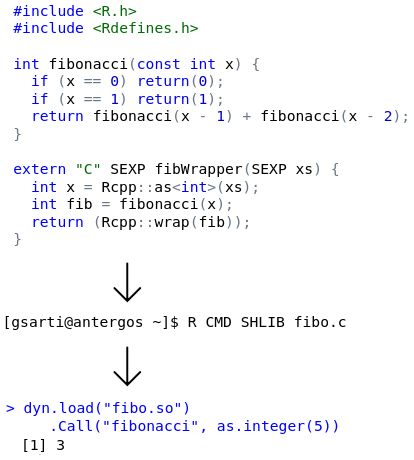
\includegraphics[width=1\textwidth]{old-way-1.png}
\end{figure} \pause
\column{0.5\textwidth}
\begin{figure}[htb]
    \centering
    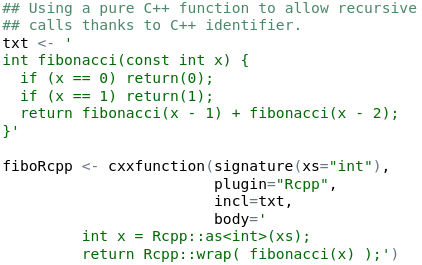
\includegraphics[width=1\textwidth]{old-way-2.png}
\end{figure} \pause
\\
\vspace{3mm}
Still using \code{as} an \code{wrap} functions from the original \code{C API} through the \code{inline} package, still not intuitive enough.
\end{columns}
\end{frame}

%-----------------------------------

\begin{frame}
\frametitle{A Simple Example: The Modern Way}
\begin{columns}
\column{0.5\textwidth}
\begin{figure}[htb]
    \centering
    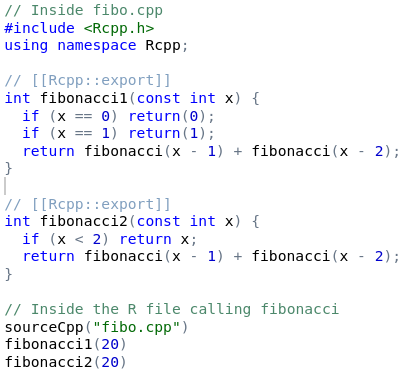
\includegraphics[width=1\textwidth]{new-way-2.png}
\end{figure} \pause
\column{0.5\textwidth}
\begin{figure}[htb]
    \centering
    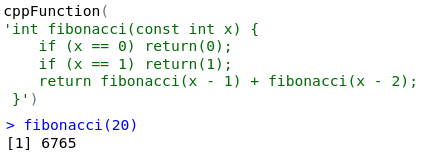
\includegraphics[width=1\textwidth]{new-way-1.png}
\end{figure} \pause
\begin{figure}[htb]
    \centering
    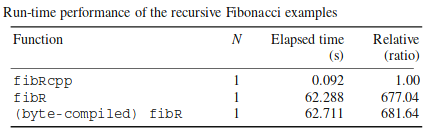
\includegraphics[width=1\textwidth]{results.png}
\end{figure} \pause
\end{columns}
\end{frame}

%-----------------------------------

\begin{frame}
\frametitle{Behind the Scenes of Rcpp Attributes}
\code{C++}11 attributes referred by \code{[[Rcpp::export]]} encapsulated the complexity of the \code{inline} package.\pause
\\
\vspace{3mm}
The new functions \code{cppFunction}, \code{sourceCpp} and \code{evalCpp} are thus much simpler. Using \code{/*** R} inside \code{C++} files is also allowed!\pause
\begin{itemize}
    \item \code{cppFunction} returns an R function which calls a wrapper in a temporary file which it also builds, which in turn  calls  the \code{C++} function we  passed  as  a  character string. \pause
    \item \code{sourceCpp} compiles, links, and loads the corresponding \code{C++} source file. \pause
\end{itemize}
\\
\vspace{3mm}
A caching mechanism ensures a single compilation of the code.
\end{frame}

%-----------------------------------

\section{Core Data Types}

% RObject parent abstract di tutte le altre classi
% IntegerVector, NumericVector, LogicalVector, CharacterVector, RawVector
%	  Parsare l'input e l'output (automatico o wrap, tipi di vettori)
%	  Named class, DataFrame
% Advanced data structures: Environment, Function, S4 e ReferenceClass

%-----------------------------------

\begin{frame}
	\frametitle{SEXP and SEXPREC}
	
Objects in \code{R} are internally represented as \code{SEXP}, a pointer to a so-called S-expression object, or \code{SEXPREC} for short (or \code{VECSXP} and \code{VECSXPREC} for vectors). \pause

\bigskip

\code{SEXPR} objects are \alert{union types} (which are sometimes called variant types). This means that depending on the particular value in an 64 bit header, different types can be represented. \pause

\bigskip

\code{SEXP} objects should be considered opaque, i.e. should be accessed only by macros provided by the \code{R API}. In this sense \code{Rcpp API} provides an higher level of abstraction 

	
	
\end{frame}	

%-----------------------------------

\begin{frame}

\frametitle{The RObject Class}

The \code{RObject} class is the basic class underlying the \code{Rcpp API}. It is the parent of all the classes we are going to see next and it is the main ingredient of the package abstraction. \pause

\bigskip

We can think of an \code{RObject} as wrapper around the \code{SEXP} structure (In fact, the \code{SEXP} is indeed the only data member of an \code{RObject})  \pause

\bigskip

The main idea is that all the functions that directly access the \code{SEXP} object are implemented in this class, this gives the user a much more transparent way to interact with \code{R} internals.

\end{frame}

%-----------------------------------
	
\begin{frame}
	
\frametitle{Numeric Vector and Integer Vector}	

Is pretty rare to instantiate a raw \code{RObject}. It is preferable to work with the derived classes which are specific for each \code{R} type. \pause

\bigskip

Templated function \code{as<>()} and class constructors with \code{R} objects as argument are used to convert a \code{SEXP} structure to the corresponding \code{Rcpp} type. The \code{SEXP} to \code{R} can be returned by using \code{wrap()}. \pause

\bigskip

Two of the most commonly used \code{Rcpp} classes are:

\begin{itemize}
	\item \alert{Numeric Vector}: corresponds to the basic \code{R} type of a numeric vector and can hold real-valued floating-point variables. \pause
	\item \alert{Integer Vector}: Provides a natural mapping from and to the standard \code{R} integer vectors.
\end{itemize}

\end{frame}

%-----------------------------------

\begin{frame}
\frametitle{Other Vector Classes}
	
Other common used vector classes are:
\begin{itemize}
	\item \alert{Logical Vector} for storing boolean values.
	\item \alert{Character Vector} for strings.
	\item \alert{Raw Vector} for raw bytes.
\end{itemize} \pause

\bigskip

Numeric and Integer matrix are also present. Vectors are actually implemented as multidimensional, their dimension can be changed by providing an attribute in the object constructor. \pause

\bigskip

Another useful feature of the vector family is the the presence of already implemented iterators, which gives full compatibility with the \code{C++} STL methods.

\end{frame}

%-----------------------------------

\begin{frame}
	\frametitle{Named and List}
The \alert{Named} class is an helper class used for setting the key side of key/value pairs. It corresponds to \code{R}'s \code{c()} map construct.
\begin{figure}
	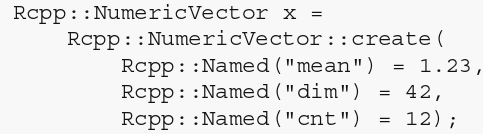
\includegraphics[width=0.6\textwidth]{named.png}
\end{figure} \pause

\bigskip

The \alert{Generic Vector} class is the equivalent of the \code{List} type in \code{R}. It can contain objects of different types, including other generic vectors. Because of its flexibility it is commonly used to parameter exchanges in either directions.

\end{frame}

%-----------------------------------

\begin{frame}
\frametitle{Function and Dataframe}

The \alert{Function} class helps us whenever we want to use an \code{R} function in \code{Rcpp}. It is possible to either pass the \code{Function} object or to retrieve it from the environment by name. \pause

\bigskip

The \alert{Dataframe} class is, much like its \code{R} counterpart, implemented as lists constrained to have elements of the same length. However, while \code{R} dataframes can \emph{recycle}, i.e. elements of the shorter columns can be repeated until a valid \code{Dataframe} structure is obtained, this is not possible in \code{Rcpp} dataframes and will raise an exception.

\end{frame}

%-----------------------------------

\begin{frame}
\frametitle{Environments}
In \code{Rcpp} the \alert{Environment} class can be used to retrieve and modify elements in an \code{R} environment. \pause

\bigskip

Environments associate a set of names to a set of values. They can be thought as named lists but with some differences: 
\begin{itemize}
	\item Every name in an environment is unique. \pause
	\item The names in an environment are not ordered.  \pause
	\item An environment has always a parent (except the empty environment). \pause
	\item Environments have reference semantics. \pause
\end{itemize} 

\bigskip

Namespaces are implemented using environments, and environment enable the use of \emph{closures} as the standard for functions in \code{R}. 
\end{frame}

%-----------------------------------

\begin{frame}
\frametitle{The R Object Oriented System}

There are three main object systems in \code{R}:
\begin{itemize}
	\item<1-> \alert{S3} implements \emph{generic-function object orientation}, different from the more common message-passing object orientation where the methods belongs to a class. Computations are still performed via methods, but a generic function decides which method to call. \code{S3} has no formal definition of classes.
	\item<2-> \alert{S4} are just \code{S3} objects with more formalism. They have a rigorous definition of attributes and inheritance, and have helper functions for defining generics and methods. 
	\item<3-> \alert{RC} implements message-passing object orientation. \code{RC} objects are also mutable: they don’t use \code{R}’s usual copy-on-modify semantics, but are modified in place. 
\end{itemize}

\end{frame}

%-----------------------------------

\begin{frame}
	\frametitle{S4 and RC}

The \alert{\code{Rcpp S4}} class allows access and modification of \code{S4} objects attributes, allowing to test if an \code{RObject} is a \code{S4}. Nevertheless, it is a good practice to manipulate the object and isolate the interesting attributes directly in \code{R}, and then carry out the computations in \code{Rcpp} using simpler types.
\bigskip

The \alert{\code{Rcpp RC}} class provides a natural interface for \code{R RC} classes. It is mostly used for mutable data-structures, particularly those that deal with graphics and stream of data. However, \code{RC} is not a common data-type and it is not firmly established in the community. 

\end{frame}

%-----------------------------------


\section{Advanced Rcpp}

% Exposing functions and classes
% Plugins e flag di compilazione
% Sugar
% 	 Tabella 8.1 del libro di Rcpp molto figa

\begin{frame}
\frametitle{Rcpp Sugar}
\code{Rcpp} provides a lot of syntactic sugar expressions to ensure that \code{C++} functions work very similarly to their \code{R} equivalents.
\code{Rcpp} sugar makes possible to write efficient \code{C++} code that looks almost identical to its R equivalent.

\begin{itemize}
    \item<1-> arithmetic and logical vectorized operators: $+, *, -, /,$ \code{pow}$, <, <=, >, >=, ==, !=, !$
    \item<2-> logical summary functions: \code{any()}, \code{all()}
    \item<3-> scalar summaries: \code{mean()}, \code{min()}, \code{max()}, \code{sum()}, \code{sd()}, ...
    \item<4-> vector views: \code{head()}, \code{tail()}, \code{rep\_len()}, ...
    \item<5-> basic math functions: \code{abs()}, \code{log()}, \code{sin()}, ... 
    \item<6-> distributions: \code{runif()}, \code{dnorm()}, ...
\end{itemize}
\end{frame}
%-----------------------------------


%---------------------------------------------------------
\begin{frame}
\frametitle{Rcpp Sugar: An Example}
\begin{columns}
\column{0.5\textwidth}
\begin{figure}[htb]
    \centering
    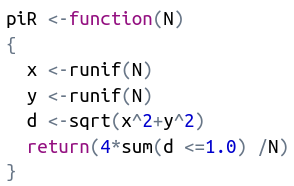
\includegraphics[width=0.8\textwidth]{sugar_piR.png}
\end{figure} \pause
\column{0.5\textwidth}
\begin{figure}[htb]
    \centering
    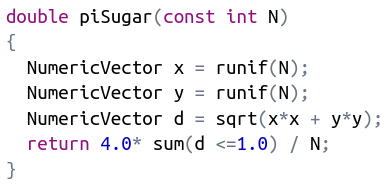
\includegraphics[width=1.1\textwidth]{sugar_piSugar.png}
\end{figure} 
\vspace{2mm}
\pause
\end{columns}
\\
\vspace{3mm}
The only difference is the type declaration and the missing operator \code{\^} in \code{C++}.

\end{frame}
%---------------------------------------------------------


%---------------------------------------------------------
\begin{frame}
\frametitle{Rcpp Sugar: Performances}

\begin{figure}[s3]
    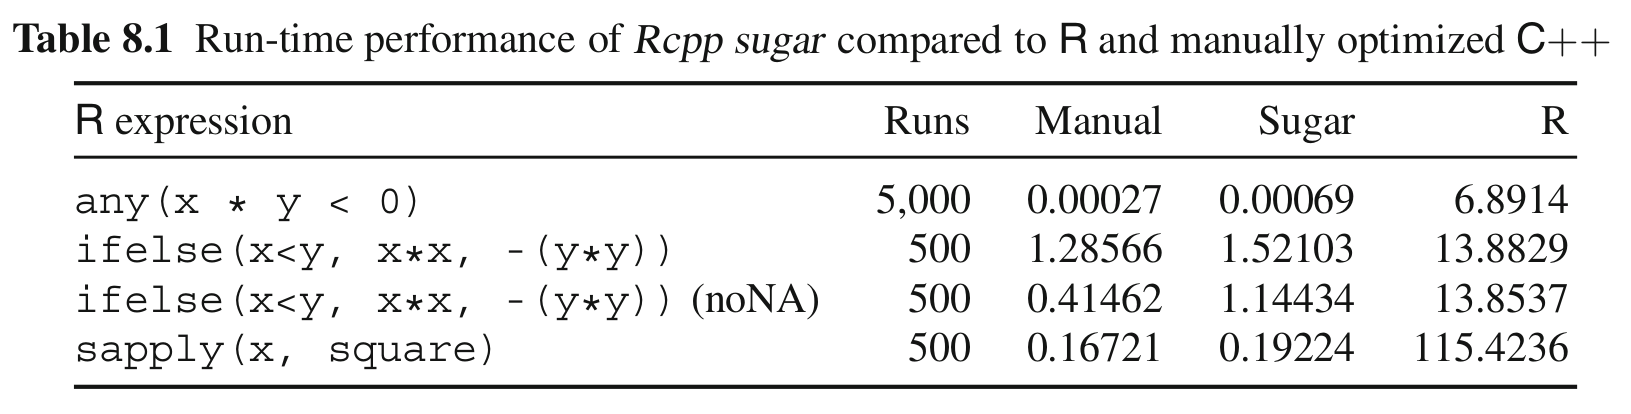
\includegraphics[width=1\textwidth]{sugar_hand_r.png}
\end{figure}

Sugar functions don't always perform like hand-written ones in \code{C++} (for now!)

\end{frame}
%---------------------------------------------------------


%-----------------------------------
\begin{frame}
\frametitle{Exposing C++ Classes to R}
We've already seen how to use \code{C++} functions in \code{R}, now we want to 
use an entire user-defined \code{C++} class in \code{R}.

\begin{itemize}
    \item<1-> Unlike functions, it does not exist an attribute shortcut for classes
    \item<2-> Anyway, it's possible to avoid writing tedious operational code. How?
    \item<3-> Thanks to the macro \code{RCPP\_MODULE}, that \code{Rcpp} provides.
    \item<4-> It can be used also for exposing functions.
    
\end{itemize}
\end{frame}
%-----------------------------------


%-----------------------------------
\begin{frame}
\frametitle{Exposing C++ Classes: An Example}

\begin{figure}[s2]
    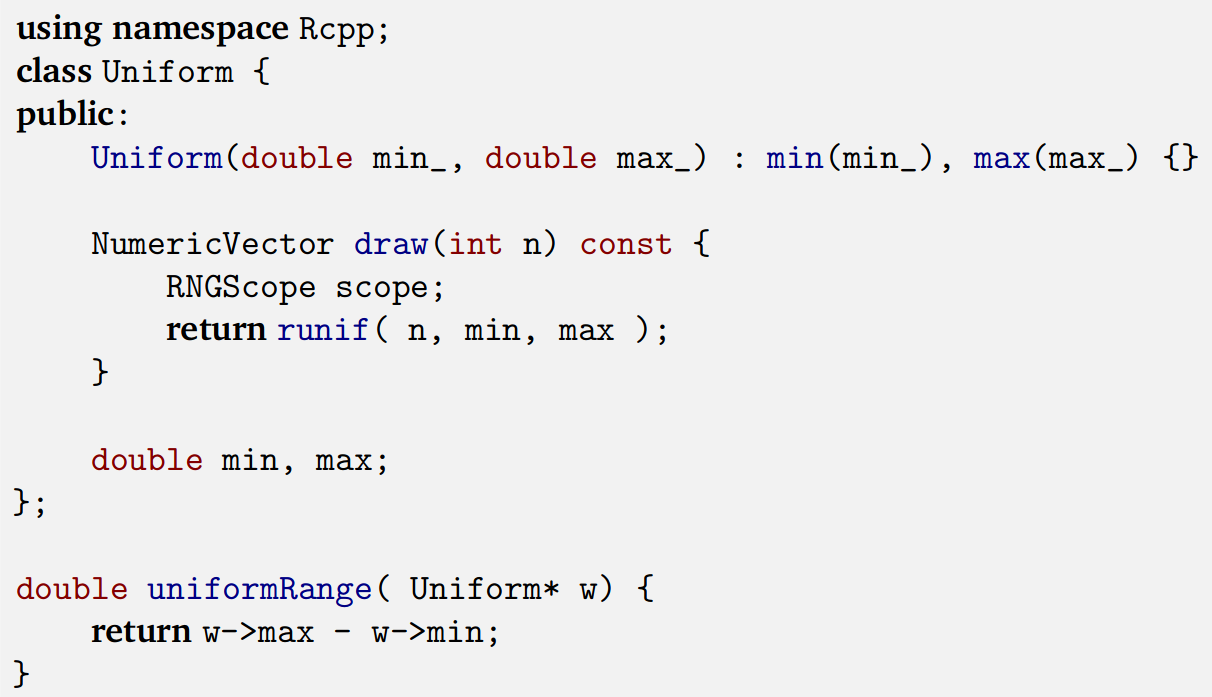
\includegraphics[width=1\textwidth]{exposing_classes_1.png}
\end{figure}
\end{frame}
%-----------------------------------


%-----------------------------------
\begin{frame}
\frametitle{Exposing C++ classes: An Example}
We just have to choose a name for the module, and declare a name for every class member.
\begin{figure}[s2]
    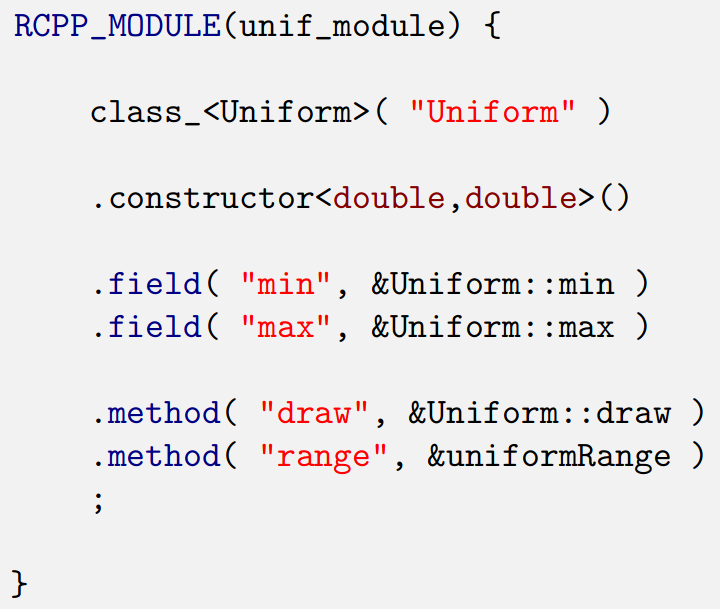
\includegraphics[width=0.65\textwidth]{exposing_classes_2.png}
\end{figure}
\end{frame}
%-----------------------------------

%-----------------------------------
\begin{frame}
\frametitle{Exposing C++ classes: An Example}
After compiling the \code{.cpp} file as a dynamic library, we load the module in \code{R}, and now it's ready to be used like a class.
\begin{figure}[s2]
    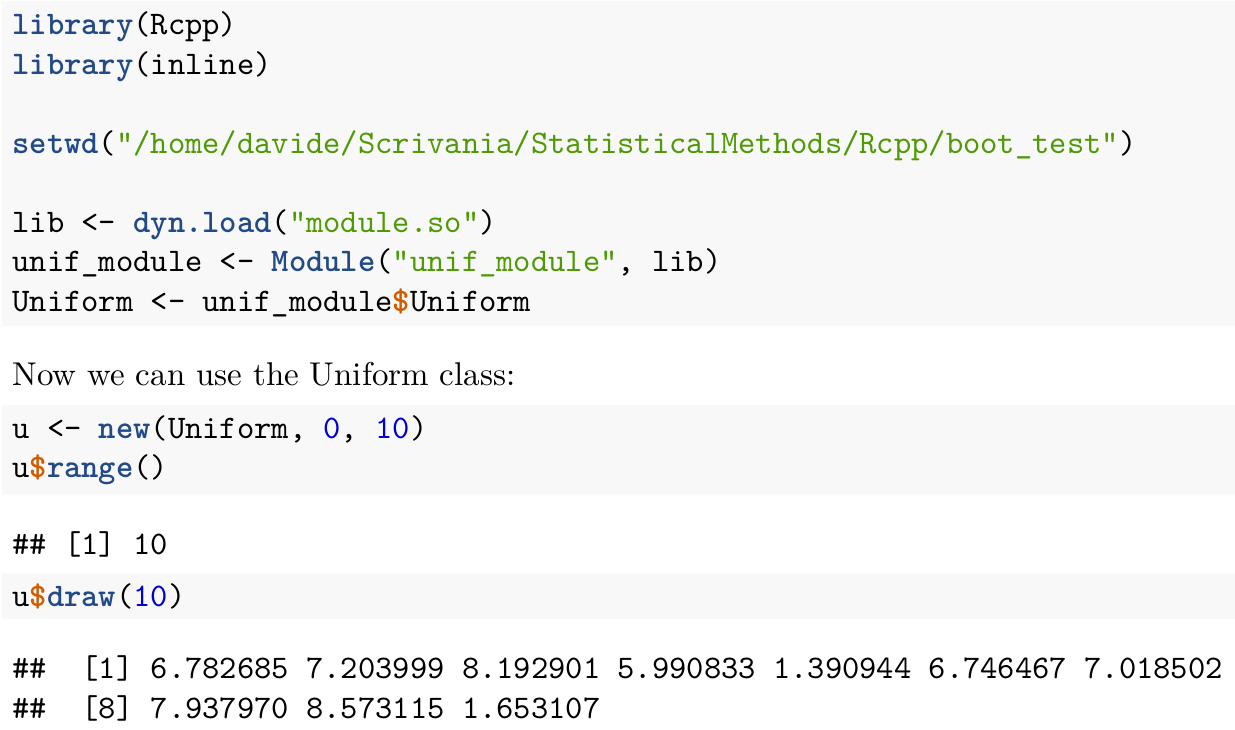
\includegraphics[width=0.95\textwidth]{exposing_classes_3.png}
\end{figure}
\end{frame}
%-----------------------------------


%-----------------------------------
\begin{frame}
\frametitle{Extending Rcpp}

Many packages are available to extend base \code{Rcpp} functionalities:
\begin{itemize}
    \item \code{Rinside}: Embedded \code{R} in \code{C++} applications. \pause
    \item \code{RcppArmadillo}: Interface to \code{Armadillo}, a linear algebra library that balances speed and ease of use. \pause
    \item \code{RcppEigen}: Interface to the \code{Eigen} library, a library suited for dealing with matrix decomposition and sparse matrices. \pause
\end{itemize}
\begin{columns}
\column{0.4\textwidth}
\begin{figure}[htb]
    \centering
    
\includegraphics[width=0.5\textwidth]{armadillo.png}
\end{figure}
\column{0.4\textwidth}
\begin{figure}[htb]
    \centering
    
\includegraphics[width=0.5\textwidth]{eigen.png}
\end{figure}
\end{columns}

\end{frame}
%-----------------------------------

%-----------------------------------
\begin{frame}
\frametitle{RcppArmadillo: An Example}
\begin{columns}
\column{0.5\textwidth}
\begin{figure}[htb]
    \centering
    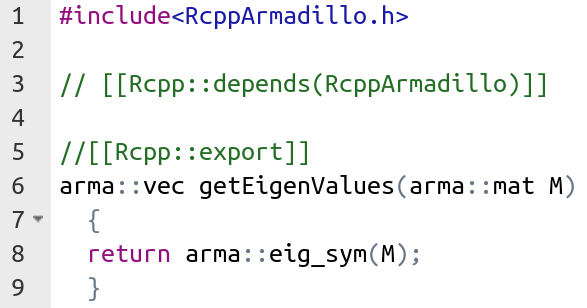
\includegraphics[width=1.1\textwidth]{armadillo_1.png}
\end{figure} \pause
\column{0.5\textwidth}
\begin{figure}[htb]
    \centering
    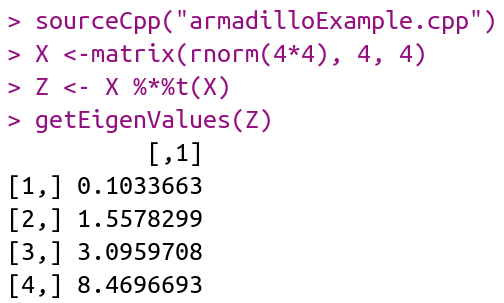
\includegraphics[width=0.9\textwidth]{armadillo_2.png}
\end{figure} \pause
\end{columns}
\\
\vspace{5mm}
Notice that using attributes it is possible to declare dependencies on other packages.

\end{frame}
%-----------------------------------


\section{Bootstrapping in Rcpp}

% Demo di bootstrap in R
% Demo di boostrap in Rcpp e miglioramento

% Insert content here
%---------------------------------------------------------
\begin{frame}
\frametitle{Bootstrap}

\begin{alertblock}{Definition}
\alert{Bootstrapping} is a type of resampling where large numbers of smaller samples of the same size are repeatedly drawn, with replacement, from a single original sample.
\end{alertblock}

\\
\vspace{3mm}
In order to show a possible use case of \code{Rcpp} in statistics, we will write a function that computes the means and the standard deviations for a set of $B$ samples bootstrapped from an original data set of size $n$.
\\
\vspace{3mm}
Since the process is iterative by definition, we expect a \code{for} loop in the implementation, which can possibly be optimized by \code{Rcpp}.
\end{frame}
%---------------------------------------------------------


%---------------------------------------------------------
\begin{frame}
\frametitle{Bootstrap, The R way}

\begin{figure}[b1]
    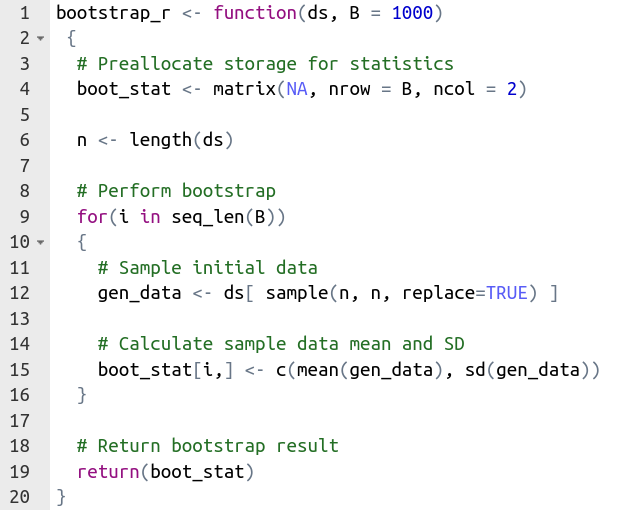
\includegraphics[width=0.7\textwidth]{bootstrap_r.png}
\end{figure}

\end{frame}
%---------------------------------------------------------

%---------------------------------------------------------
\begin{frame}
\frametitle{Bootstrap, The C++ way}

\begin{figure}[b2]
    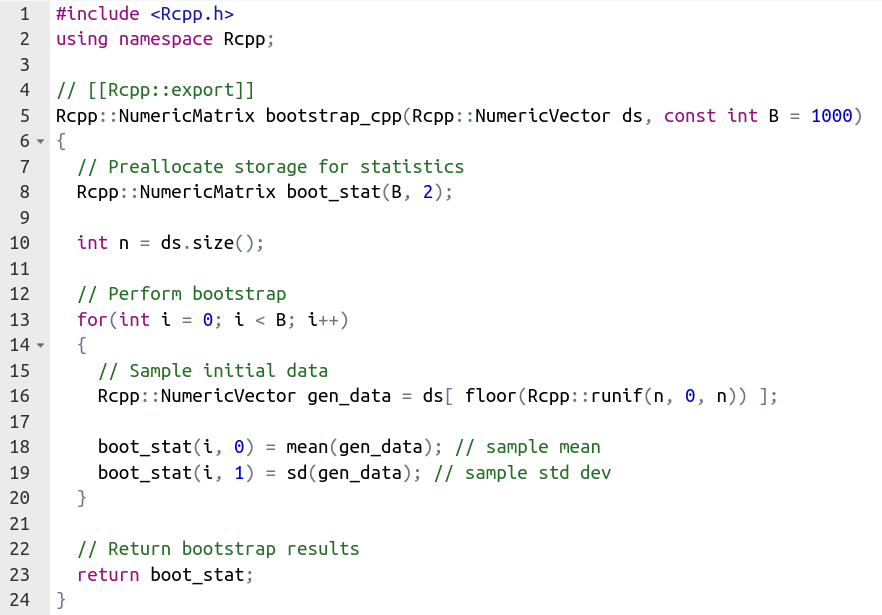
\includegraphics[width=0.9\textwidth]{bootstrap_cpp.png}
\end{figure}

\end{frame}
%---------------------------------------------------------


%---------------------------------------------------------
\begin{frame}
\frametitle{Bootstrap Performances}

\begin{figure}[b3]
    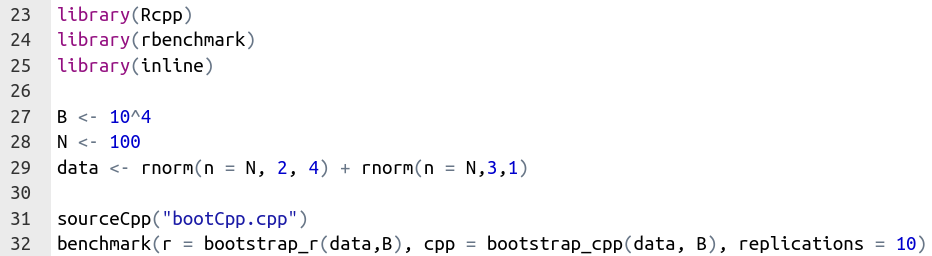
\includegraphics[width=1 \textwidth]{bootstrap_call.png}
\end{figure}

\begin{figure}[b4]
    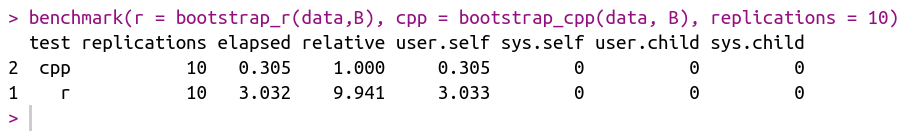
\includegraphics[width=1 \textwidth]{bootstrap_r_vs_cpp.png}
\end{figure}

Our \code{Rcpp} approach is almost ten times faster!

\end{frame}

%---------------------------------------------------------

\section{References}

\begin{frame}[allowframebreaks]
\frametitle{References}
    \bibliographystyle{amsalpha}
    \bibliography{biblio.bib}
    \nocite{*}
\end{frame}
\end{document}